% Compile this file separately to produce the supplementary tables PDF.
\documentclass[11pt]{article}
\usepackage[margin=1in]{geometry}
\usepackage[T1]{fontenc}
\usepackage[utf8]{inputenc}
\usepackage{lmodern}
\usepackage{booktabs}
\usepackage{graphicx}
\usepackage{adjustbox}
\usepackage{threeparttable}
\usepackage{longtable}
\usepackage[hidelinks]{hyperref}
\renewcommand{\arraystretch}{1.10}
\newcommand{\Pzero}{\textit{P0}}
\newcommand{\Pone}{\textit{P1}}
\newcommand{\Ptwo}{\textit{P2}}
\begin{document}
\begin{center}
{\Large \textbf{Supplementary material}}\\[0.4em]
{\large Does Daily Workload and Wellness Monitoring Add Incremental Value Beyond a Personalised Autoregressive Baseline for Next-Day Readiness?}
\end{center}
\vspace{1em}
\renewcommand{\thetable}{S\arabic{table}}
\setcounter{table}{0}

\begin{table}[htbp]
\centering
\caption{Model-specific full-pipeline tuning in source-team 2020 data. Candidate penalties were $\alpha=0,0.0001,0.001,0.01,0.1,1,10,100,1000,10000,100000$ and were evaluated in three expanding chronological folds. Selection used weighted validation MAE after reset sequential residual adaptation.}
\scriptsize
\begin{tabular}{llrrr}
\toprule
Source team & Model & Selected $\alpha$ & Weighted validation MAE & Validation pairs \\
\midrule
Team A & P0 & 1000 & 0.797 & 1,792 \\
Team A & P1 & 1000 & 0.786 & 1,792 \\
Team A & P2 & 1000 & 0.783 & 1,792 \\
Team B & P0 & 1000 & 0.566 & 1,064 \\
Team B & P1 & 1000 & 0.576 & 1,064 \\
Team B & P2 & 1000 & 0.577 & 1,064 \\
\bottomrule
\end{tabular}
\end{table}

\begin{table}[htbp]
\centering
\caption{Residual-window and reduced-monitoring sensitivity analyses. Positive values indicate higher MAE for the candidate model than for the readiness-history baseline.}
\scriptsize
\resizebox{\textwidth}{!}{%
\begin{tabular}{lrrl}
\toprule
Evaluation setting & Residual window & Test pairs & Candidate$-$\Pzero{} MAE (95\% CI) \\
\midrule
Within Team A: 2020$\rightarrow$2021 & 14 & 5,881 & +0.010 (-0.003 to +0.027) \\
Within Team A: 2020$\rightarrow$2021 & 28 & 5,881 & +0.007 (-0.005 to +0.023) \\
Within Team A: 2020$\rightarrow$2021 & 56 & 5,881 & +0.004 (-0.007 to +0.020) \\
Within Team B: 2020$\rightarrow$2021 & 14 & 2,483 & +0.021 (-0.003 to +0.049) \\
Within Team B: 2020$\rightarrow$2021 & 28 & 2,483 & +0.018 (-0.005 to +0.047) \\
Within Team B: 2020$\rightarrow$2021 & 56 & 2,483 & +0.014 (-0.011 to +0.043) \\
Team A 2020$\rightarrow$Team B 2021 & 14 & 2,483 & +0.028 (+0.001 to +0.060) \\
Team A 2020$\rightarrow$Team B 2021 & 28 & 2,483 & +0.022 (-0.005 to +0.053) \\
Team A 2020$\rightarrow$Team B 2021 & 56 & 2,483 & +0.017 (-0.012 to +0.052) \\
Team B 2020$\rightarrow$Team A 2021 & 14 & 5,881 & +0.004 (-0.007 to +0.017) \\
Team B 2020$\rightarrow$Team A 2021 & 28 & 5,881 & +0.004 (-0.007 to +0.016) \\
Team B 2020$\rightarrow$Team A 2021 & 56 & 5,881 & -0.000 (-0.009 to +0.010) \\
Within Team A: 2020$\rightarrow$2021 & 28 (P2) & 5,881 & +0.011 (-0.002 to +0.027) \\
Within Team B: 2020$\rightarrow$2021 & 28 (P2) & 2,483 & +0.017 (-0.006 to +0.044) \\
Team A 2020$\rightarrow$Team B 2021 & 28 (P2) & 2,483 & +0.023 (-0.001 to +0.052) \\
Team B 2020$\rightarrow$Team A 2021 & 28 (P2) & 5,881 & +0.002 (-0.007 to +0.013) \\
\bottomrule
\end{tabular}%
}
\end{table}

\begin{table}[htbp]
\centering
\caption{Performance and linear calibration diagnostics under the primary 28-observation residual-history window. The intercept and slope are from regressions of observed readiness on predicted readiness.}
\scriptsize
\resizebox{\textwidth}{!}{%
\begin{tabular}{llrrrrrrrr}
\toprule
Evaluation setting & Model & $\alpha$ & MAE & RMSE & Bias & $R^2$ & Intercept & Slope & Within $\pm1$ point \\
\midrule
Within Team A: 2020$\rightarrow$2021 & \Pzero & 1000 & 0.717 & 1.031 & 0.012 & 0.568 & 0.472 & 0.928 & 75.9\% \\
Within Team A: 2020$\rightarrow$2021 & \Pone & 1000 & 0.724 & 1.031 & 0.032 & 0.568 & 0.504 & 0.920 & 76.0\% \\
Within Team B: 2020$\rightarrow$2021 & \Pzero & 1000 & 0.619 & 0.965 & 0.028 & 0.486 & 0.624 & 0.908 & 81.1\% \\
Within Team B: 2020$\rightarrow$2021 & \Pone & 1000 & 0.637 & 0.956 & 0.031 & 0.496 & 0.545 & 0.919 & 80.9\% \\
Team A 2020$\rightarrow$Team B 2021 & \Pzero & 1000 & 0.618 & 0.962 & 0.029 & 0.490 & 0.502 & 0.925 & 81.3\% \\
Team A 2020$\rightarrow$Team B 2021 & \Pone & 1000 & 0.640 & 0.969 & 0.058 & 0.482 & 0.525 & 0.918 & 81.1\% \\
Team B 2020$\rightarrow$Team A 2021 & \Pzero & 1000 & 0.718 & 1.034 & 0.012 & 0.565 & 0.551 & 0.916 & 75.7\% \\
Team B 2020$\rightarrow$Team A 2021 & \Pone & 1000 & 0.722 & 1.031 & 0.017 & 0.567 & 0.531 & 0.918 & 76.0\% \\
\bottomrule
\end{tabular}%
}
\end{table}

\begin{table}[htbp]
\centering
\caption{Player-day eligibility flow from the complete calendar panel to the primary complete-case analytic cohort.}
\scriptsize
\resizebox{\textwidth}{!}{%
\begin{tabular}{lrrrrrr}
\toprule
Step & Overall player-days & Overall players & Team A player-days & Team A players & Team B player-days & Team B players \\
\midrule
Full calendar player-day panel & 36,550 & 50 & 19,737 & 27 & 16,813 & 23 \\
Observed next-day readiness & 16,997 & 50 & 11,022 & 27 & 5,975 & 23 \\
Observed current-day and next-day readiness & 14,631 & 50 & 9,722 & 27 & 4,909 & 23 \\
Plus available 7-day load history & 14,631 & 50 & 9,722 & 27 & 4,909 & 23 \\
Plus complete current-day wellness & 14,582 & 50 & 9,693 & 27 & 4,889 & 23 \\
Primary complete-case analytic cohort (7-day history) & 14,582 & 50 & 9,693 & 27 & 4,889 & 23 \\
\bottomrule
\end{tabular}%
}
\end{table}

\begin{table}[htbp]
\centering
\caption{Missingness of current-day readiness and wellness variables in the calendar player-day panel, by team and year. Values are percentages of player-days with missing values.}
\scriptsize
\resizebox{\textwidth}{!}{%
\begin{tabular}{lrrrrrrr}
\toprule
Team-year & Readiness & Fatigue & Mood & Sleep duration & Sleep quality & Soreness & Stress \\
\midrule
Team A, 2020 & 56.2 & 56.2 & 56.2 & 56.2 & 56.2 & 56.2 & 56.2 \\
Team A, 2021 & 32.1 & 32.1 & 32.1 & 32.2 & 32.1 & 32.1 & 32.1 \\
Team B, 2020 & 67.3 & 67.3 & 67.3 & 67.3 & 67.3 & 67.3 & 67.3 \\
Team B, 2021 & 61.6 & 61.6 & 61.6 & 61.6 & 61.6 & 61.6 & 61.6 \\
\bottomrule
\end{tabular}%
}
\end{table}

\begin{table}[htbp]
\centering
\caption{Missingness-aware full-pipeline tuning in source-team 2020 data. The full model used source-training median imputation and wellness-specific missingness indicators.}
\scriptsize
\begin{tabular}{llrrr}
\toprule
Source team & Model & Selected $\alpha$ & Weighted validation MAE & Validation pairs \\
\midrule
Team A & P0 & 1000 & 0.797 & 1,796 \\
Team A & P1m & 1000 & 0.787 & 1,796 \\
Team B & P0 & 1000 & 0.565 & 1,065 \\
Team B & P1m & 1000 & 0.575 & 1,065 \\
\bottomrule
\end{tabular}
\end{table}

\begin{table}[htbp]
\centering
\caption{Missingness-aware sensitivity analysis in the broader cohort with observed current and next-day readiness and 7-day load history. Positive values indicate higher MAE for the imputed full model (P1m) than for the readiness-history baseline.}
\scriptsize
\resizebox{\textwidth}{!}{%
\begin{tabular}{lrrrr}
\toprule
Evaluation setting & Test pairs & P0 MAE & P1m MAE & P1m$-$P0 MAE (95\% CI) \\
\midrule
Within Team A: 2020$\rightarrow$2021 & 5,903 & 0.716 & 0.723 & +0.008 (-0.004 to +0.025) \\
Within Team B: 2020$\rightarrow$2021 & 2,497 & 0.617 & 0.636 & +0.020 (-0.006 to +0.049) \\
Team A 2020$\rightarrow$Team B 2021 & 2,497 & 0.616 & 0.639 & +0.024 (-0.003 to +0.059) \\
Team B 2020$\rightarrow$Team A 2021 & 5,903 & 0.716 & 0.720 & +0.004 (-0.006 to +0.016) \\
\bottomrule
\end{tabular}%
}
\end{table}






\begin{figure}[htbp]
\centering
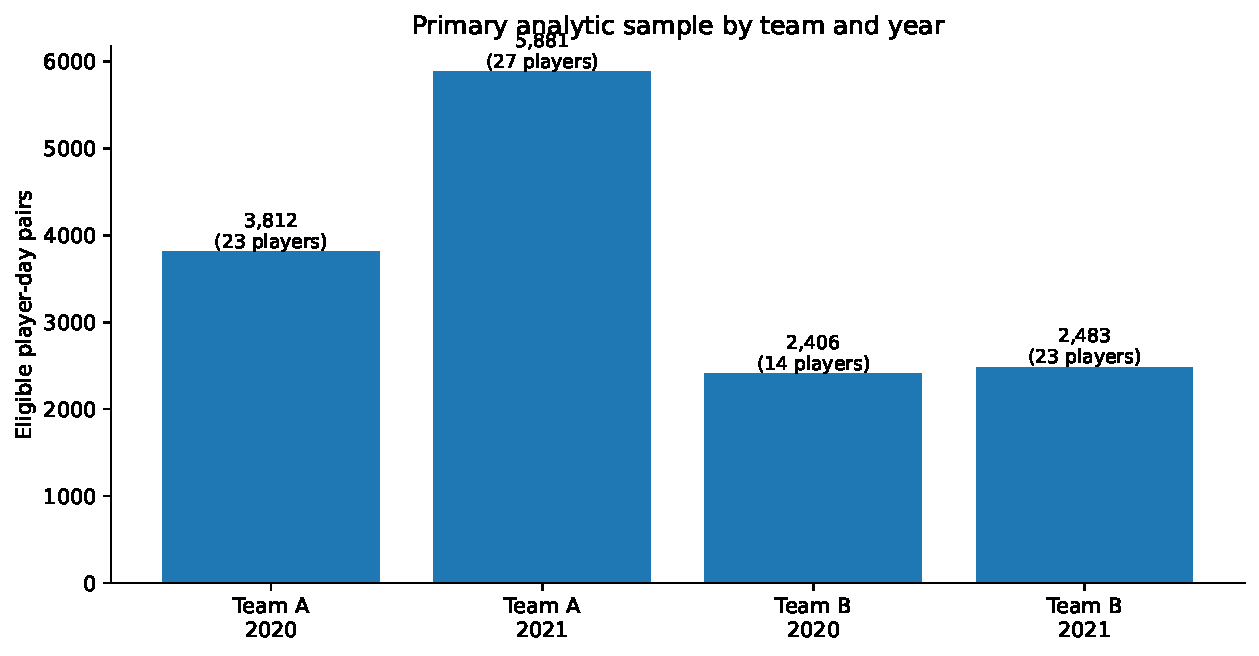
\includegraphics[width=0.80\textwidth]{figures/FigureS1_analytic_sample.pdf}
\caption{Primary analytic sample by team and year. Labels show the number of eligible player-day pairs and contributing players.}
\end{figure}

\begin{figure}[htbp]
\centering
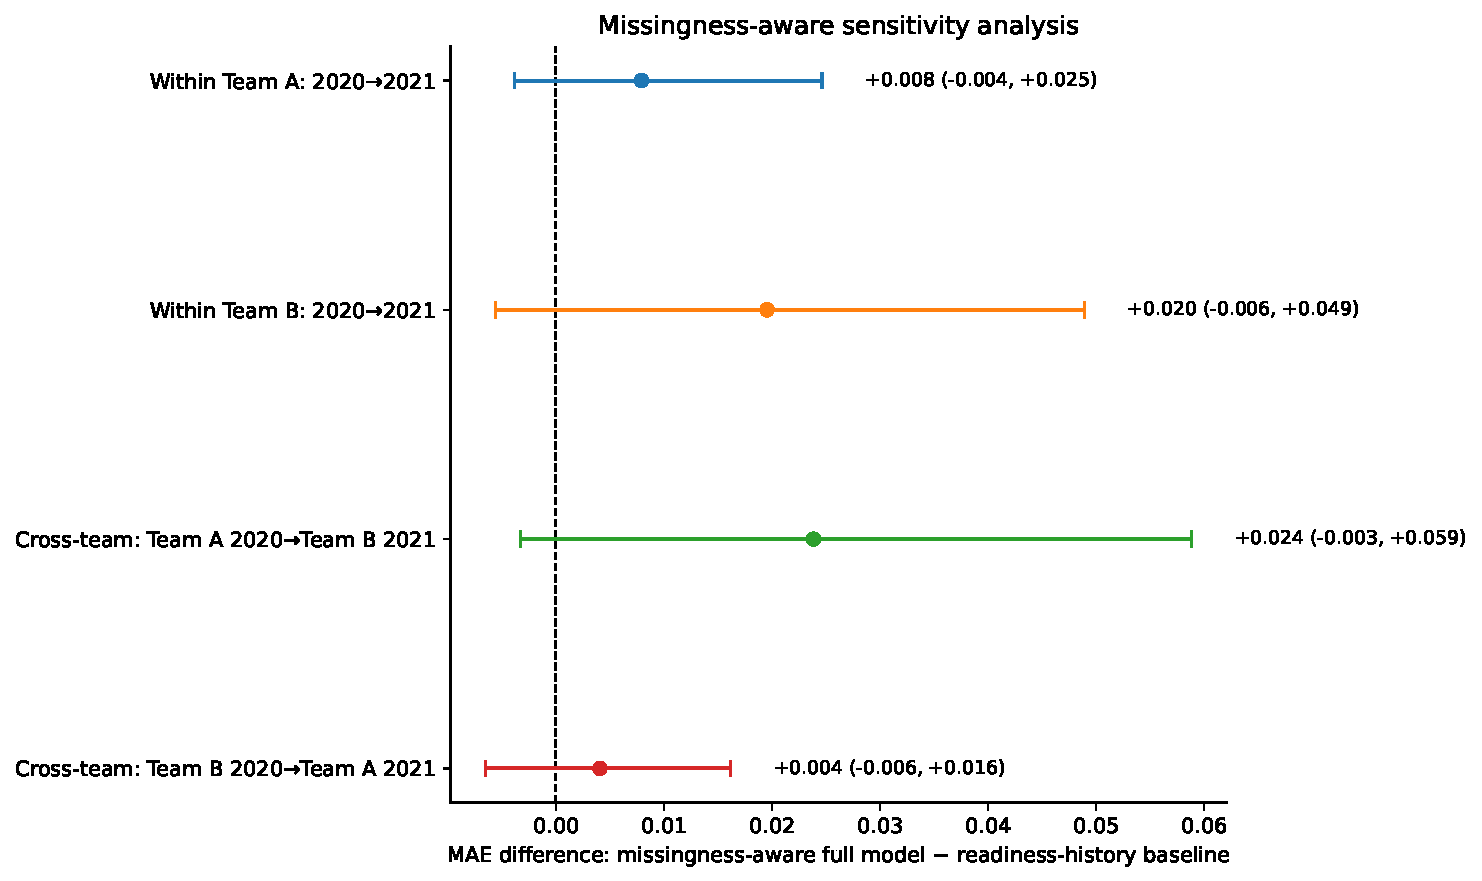
\includegraphics[width=0.88\textwidth]{figures/FigureS2_missingness_aware_incremental_value.pdf}
\caption{Missingness-aware sensitivity analysis in the broader analytic cohort. The full model used source-training median imputation and wellness-specific missingness indicators. Positive values indicate higher MAE than the readiness-history baseline.}
\end{figure}

\begin{figure}[htbp]
\centering
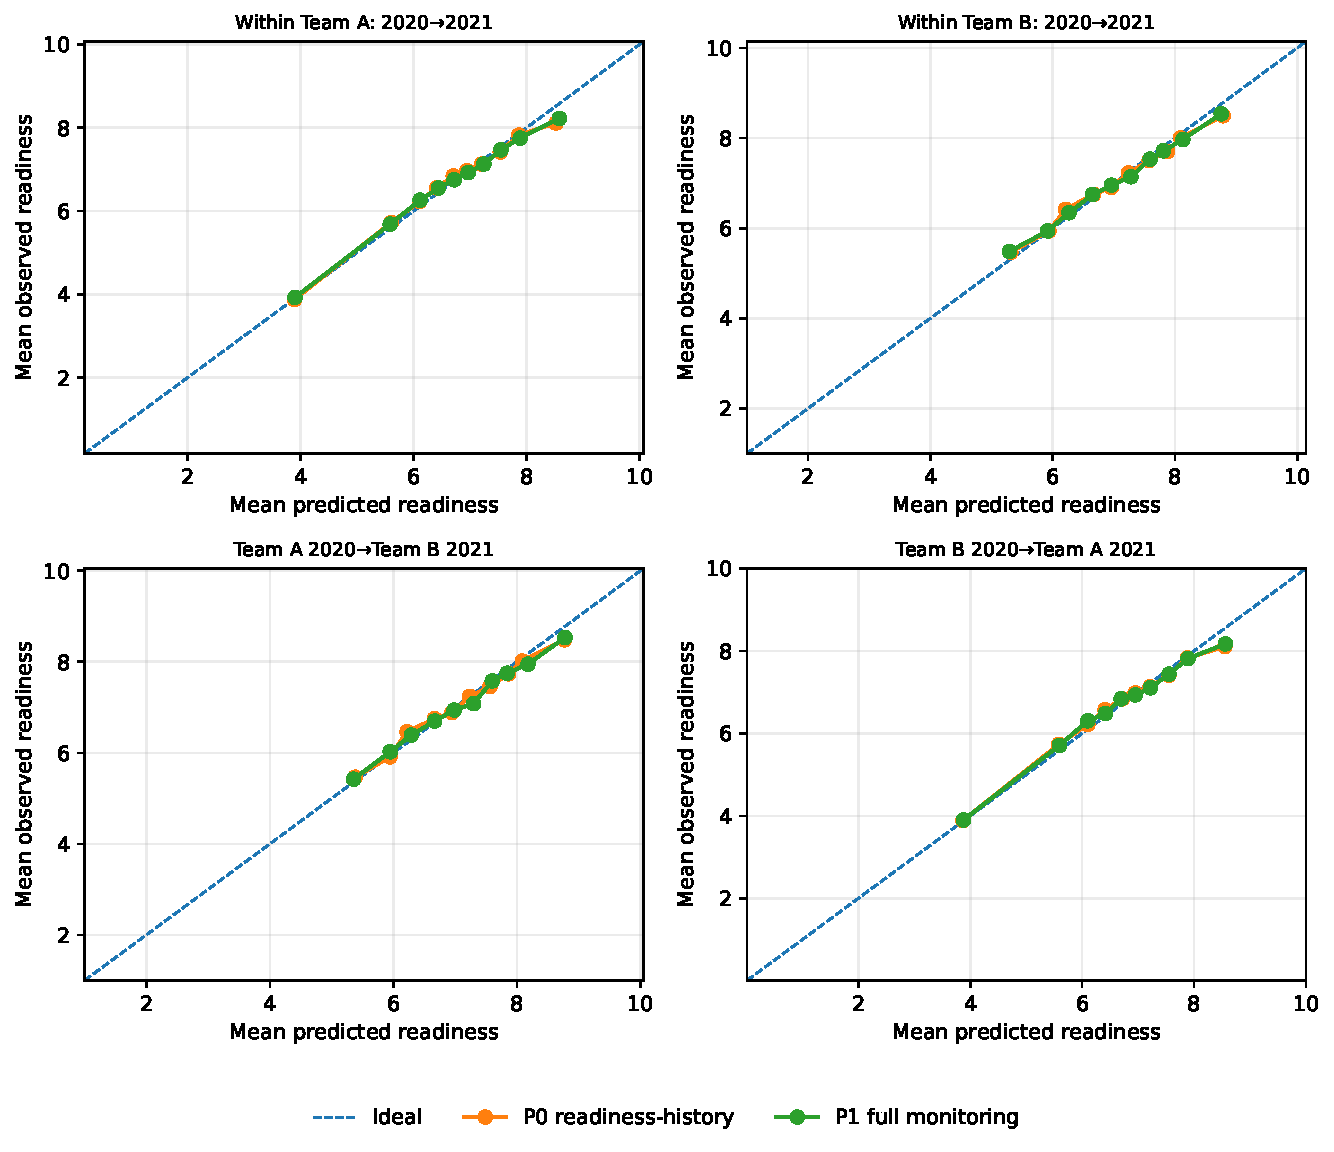
\includegraphics[width=0.95\textwidth]{figures/FigureS3_calibration_curves.pdf}
\caption{Decile-based calibration curves for \Pzero and \Pone under the primary 28-observation sequential residual-history window. Points show mean observed readiness within prediction-rank bins; the dashed line indicates ideal agreement.}
\end{figure}

\begin{figure}[htbp]
\centering
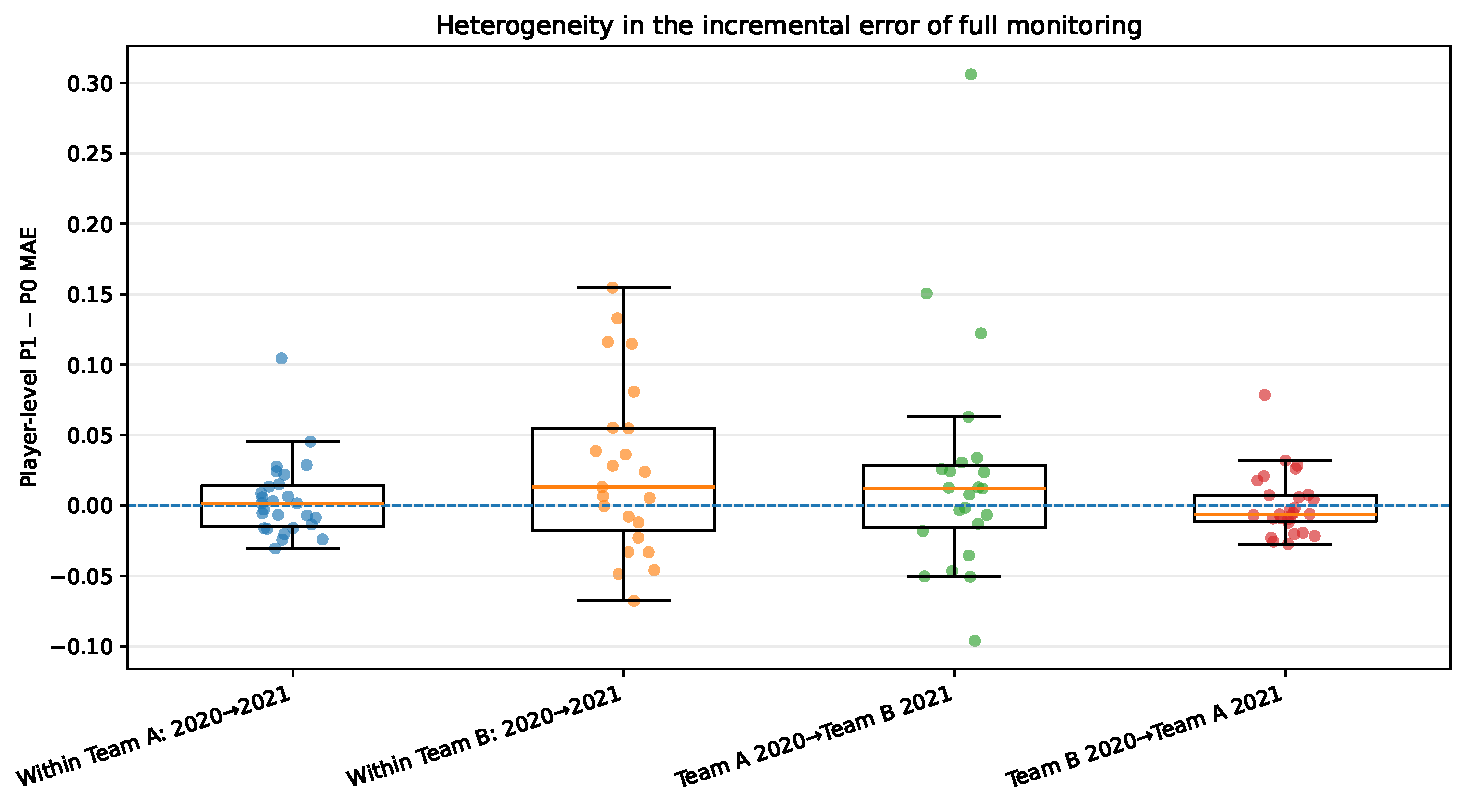
\includegraphics[width=0.88\textwidth]{figures/FigureS4_player_level_incremental_error.pdf}
\caption{Player-level heterogeneity in full-monitoring incremental MAE. Each point is one player. Positive values indicate higher MAE for \Pone than for \Pzero. Boxplots summarize player-level distributions within each evaluation setting.}
\end{figure}

\end{document}
